\chapter{Data Exploration Visualisation}\
\section{Theory}
A \textbf{Dataset} is a collection of data with a tabular representation includes rows and columns. The size of the dataset has a huge impact on the choice of the analyses, not always we can use certain algorithms because require considerable resources but there are solutions to reduce the size the cardinality preserving the completeness of the data.

Each column of the dataset represents on attribute or \textbf{feature} and every rows is a different sample, we can analyse attribute independently with their measurement, type and domain. To gain some information, starting from a theoretical distribution we use the min, max, avg, mean value, standard deviation or mathematical function.

To represent visual analyses for the univariate we use the histogram to show the distribution that can be classified as discrete probability function described by \textbf{probability mass function (PMF)} or continuous probability function described by \textbf{probability density function (PDF)}. But to be consistent and have better visualization we can't use the raw histogram so with the kernel density estimation (KDE) we can estimate continuous PDF based on samples
\begin{figure}[H]
    \centering
    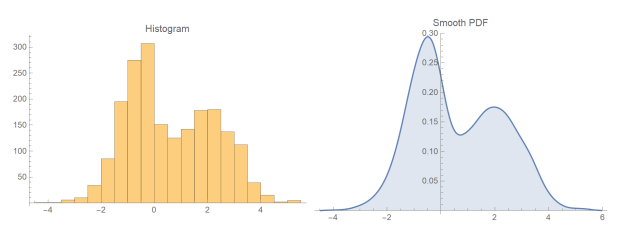
\includegraphics[scale=0.75]{images/DataExplVis/KernelDF.png}
    \caption{Caption}
    \label{fig:enter-label}
\end{figure}
To compute that we estimate f as the weighted average of neighboring observed data where the weight is defined by the kernel function, such that closer points are given higher weights and the estimated function is continuous and ‘smooth’.
\begin{center}
    $ f_{h}(x) = \frac{1}{m} \sum\limits_{i=1}^m K_{h} (x-x_{i})$
\end{center}

So KDE can produce a plot that is less cluttered and more interpretable but introduce some distortion on the data.

Cumulative distribution function (CDF) is needed to observe how the samples are distributed in different interval so to compute that we have to integrate the function from $ - \infty$ to $x$. This is very heavy in huge dataset so we can use Empirical Cumulative Distribution function (ECDF) that is an estimate of CDF that generates points in the sample. The ECDF is a step function that jumps up by 1/m at each of the m data points

\begin{figure}[H]
    \centering
    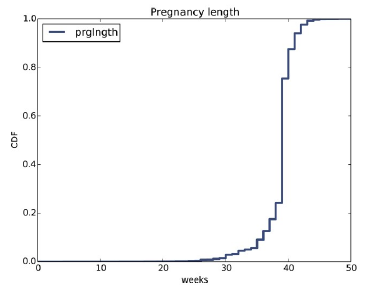
\includegraphics{images/DataExplVis/ECDF.png}
    \caption{Example of ECDF}
    \label{fig:enter-label}
\end{figure}

Percentiles indicates the value below which given percentage of observation in a group of observation falls and similarly there is the boxplot visualization. This 2 are standardized way of displaying the distribution data based on a summary values.
The boxplot can be a little tricky and this is the various part that composed it:
\begin{itemize}
    \item median: (Q2/50th Percentile): the middle value of the attribute.
    \item first quartile (Q1/25th Percentile): the middle number between the smallest number (not the “minimum”) and the median of the attribute.
    \item third quartile (Q3/75th Percentile): the middle value between the median and the highest value (not the “maximum”) of the attribute.
    \item interquartile range (IQR): 25th to the 75th percentile.
    \item whiskers (shown in blue)
    \item \textbf{outliers} (shown as green circles)
\end{itemize}

\begin{figure}[H]
    \begin{subfigure}{.5\textwidth}
        \centering
        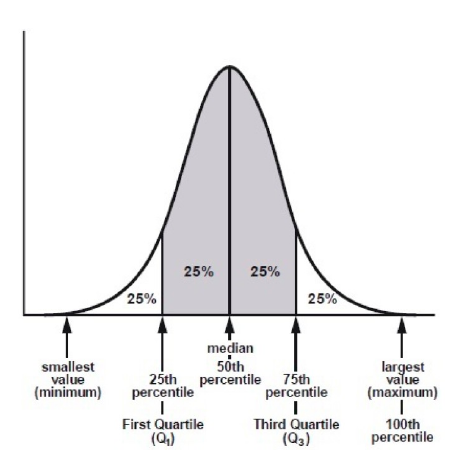
\includegraphics[width=.6\linewidth]{images/DataExplVis/Percentile.png}
        \caption{Percentile}
        \label{fig:sub1}
    \end{subfigure}
    \begin{subfigure}{.5 \textwidth}
        \centering
        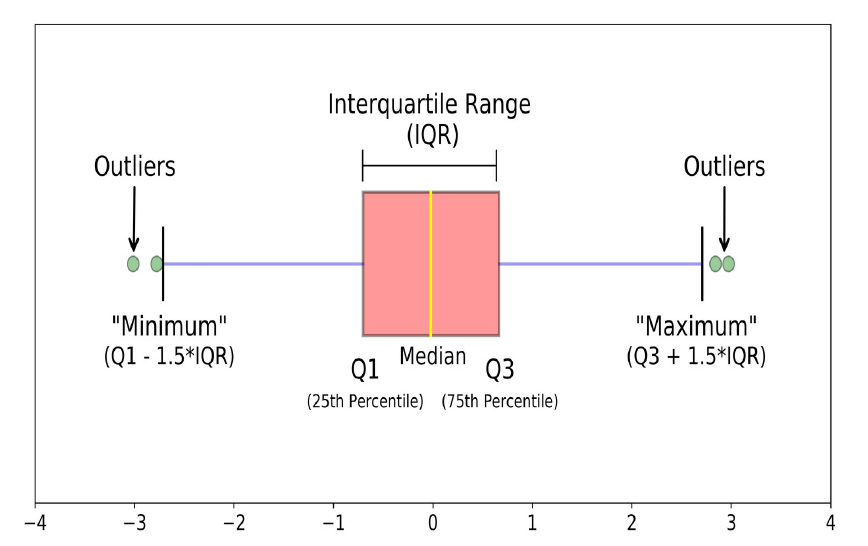
\includegraphics[width=.8\linewidth]{images/DataExplVis/Boxplot.png}
        \caption{Boxplot}
        \label{fig:sub1}
    \end{subfigure}
    \caption{Example of Percentile and Boxplot}
\end{figure}

The \textbf{Outliers} are extreme values that might be an errors in measurement and recording or an accurate reports of rare events. The best way to define/handle outliers depends on “domain knowledge” because it depends on what analysis you are planning to address.
Outlier can be detected by Generalized Extreme Studentized Deviate (GESD) but that can only be used in data set that follows a normal distribution. Another method to detect is DBSCAN that is based on a density clustering non-parametric algorithm.

However a dataset usually includes different features so the relationship between them have a key role to describe the entire dataset, this is called \textbf{correlation}. This is useful during the data exploration phase and to analyse specific data correlation because highly correlated features could be removed simplifying the performance of data driven algorithms

The simplest way to visually check for a relationship between 2 variables is a scatter plot, but to have a better comprehension  of the data we have to add some jitter or alpha parameters in order to retrieve density information

\begin{figure}[H]
    \begin{subfigure}{.5\textwidth}
        \centering
        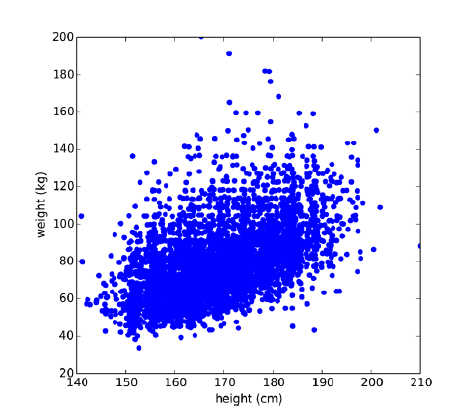
\includegraphics[width=.6\linewidth]{images/DataExplVis/Scatter1.png}
        \caption{Scatter with jitter}
        \label{fig:sub1}
    \end{subfigure}
    \begin{subfigure}{.5 \textwidth}
        \centering
        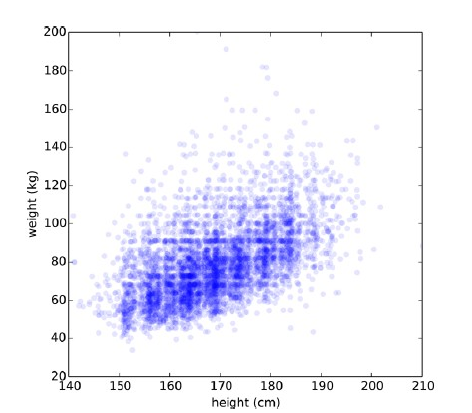
\includegraphics[width=.6\linewidth]{images/DataExplVis/Scatter2.png}
        \caption{Scatter with transparency}
        \label{fig:sub1}
    \end{subfigure}
    \caption{Example of Scatterplot}
\end{figure}

Moreover we can use scatterplot percentiles with every line that represents one percentile to focus on the main data and not the outlier.

A \textbf{correlation} is a statistic intended to quantify the strength of the relationship between two variables. Possible way to compute correlations are:
\begin{itemize}
    \item Covariance: is a measure of the joint variability of two random variables. In order to compare two variables, they must have the same unit of measurement or normalized
    \item Pearson: Solves the problem of normalization but can only detects linear correlation
    \item Spearman
\end{itemize}
The formulas for the correlation are:
\begin{center}
    $corr(x,y)=  \dfrac{covariance(x,y)}{sd(x) * sd(y)}  $\\
    $covariance(x,y) = \dfrac{1}{n-1} \sum\limits_{k=1}^n (x_{k} - \overline{x} )(y_{k} - \overline{y} )$\\
    $standard\_deviation(x)= sd(x)= \sigma(x)= \sqrt{\dfrac{1}{n-1} \sum\limits_{k=1}^n (x_{k} - \overline{x} )^2 } $\\
    $standard\_deviation(y)= sd(x)= \sigma(y)= \sqrt{\dfrac{1}{n-1} \sum\limits_{k=1}^n (y_{k} - \overline{y} )^2 } $\\
    $ \overline{x}$ and $\overline{y} $ are the mean of all x and y samples calculated with $\overline{x} = \dfrac{1}{n} \sum\limits_{k=1}^n  x_{k} $
\end{center}
Pearson is only for linear correlation and have result between {-1;1} and we use Spearman's Rank Correlation, that assesses how the relationship between two variables can be transformed into  a rank and can be described using a monotonic function and the advantage is that in some cases the Spearman index allows to find a correlation when the Pearson index returns a value close to 0.
The formulas changes to:
\begin{center}
    $ r_s =  \rho_{(R(x),R(y))} = \dfrac{cov(R(x),R(y))}{\sigma_{R(x)} \sigma_{R(y)}}$\\
    if all m ranks are distinct we can use $ r_s = 1 - \dfrac{6 \sum (R(X_i) - R(Y_i))^2}{m(m^2 -1)}$
\end{center}
Other data visualization are:
\begin{itemize}
    \item heatmap
    \item Word Cloud
    \item PCA
    \item T-SNE
\end{itemize}

    



